\nnarticleheader{Gabriel’s Horn Paradox}{Mitav Nayak, Haverford '22}
\noindent
\textbf{Introduction}

	Perplexing yet intriguing, “Gabriel’s Horn” is a geometric shape formed by rotating the graph of $f(x)=\frac{1}{x}$ about the x-axis that has fascinated mathematicians for centuries. Evangelista Torricelli, an Italian mathematician and physicist, was the first to examine the shape during the 1600s. Torricelli studied under Galileo, and gained fame for his development of the barometer. Furthermore, Torricelli worked with infinite series, contributing toward the proof of the sum for the telescoping series. He was a prominent mathematical figure in the seventeenth century, and his work surrounding Gabriel’s Horn sparked debates surrounding the nature of infinity in the years after his death.

	Gabriel’s Horn – also known as Torricelli’s Trumpet – is a figure with a finite volume but an infinite surface area. In other words, if a painter was tasked with filling the horn with paint, he would need a finite amount of paint. However, if the painter was tasked with painting the entire inside or outside surface, it would be impossible, as he would need an infinite amount of paint. This paradox, known as the painter’s paradox, can be shown by solving for both the volume and surface area of the figure.
\\
%add first image here
\renewcommand{\thefigure}{1}
\begin{figure}[h!]
  \begin{center}
    
\includegraphics[scale=.25]{nayak_horn}
    \caption{Gabriel's Horn}
    \label{fig:1} 
  \end{center}
\end{figure}

\newpage
\noindent
\textbf{Mathematical Explanation}

	Consider the graph $f(x)=\frac{1}{x}$ (Figure 2). Now, consider this graph on the interval $[1,\infty)$ rotated about the x-axis (Figure 3).
	
\renewcommand{\thefigure}{2}
\begin{figure}[h]
  \begin{center}
    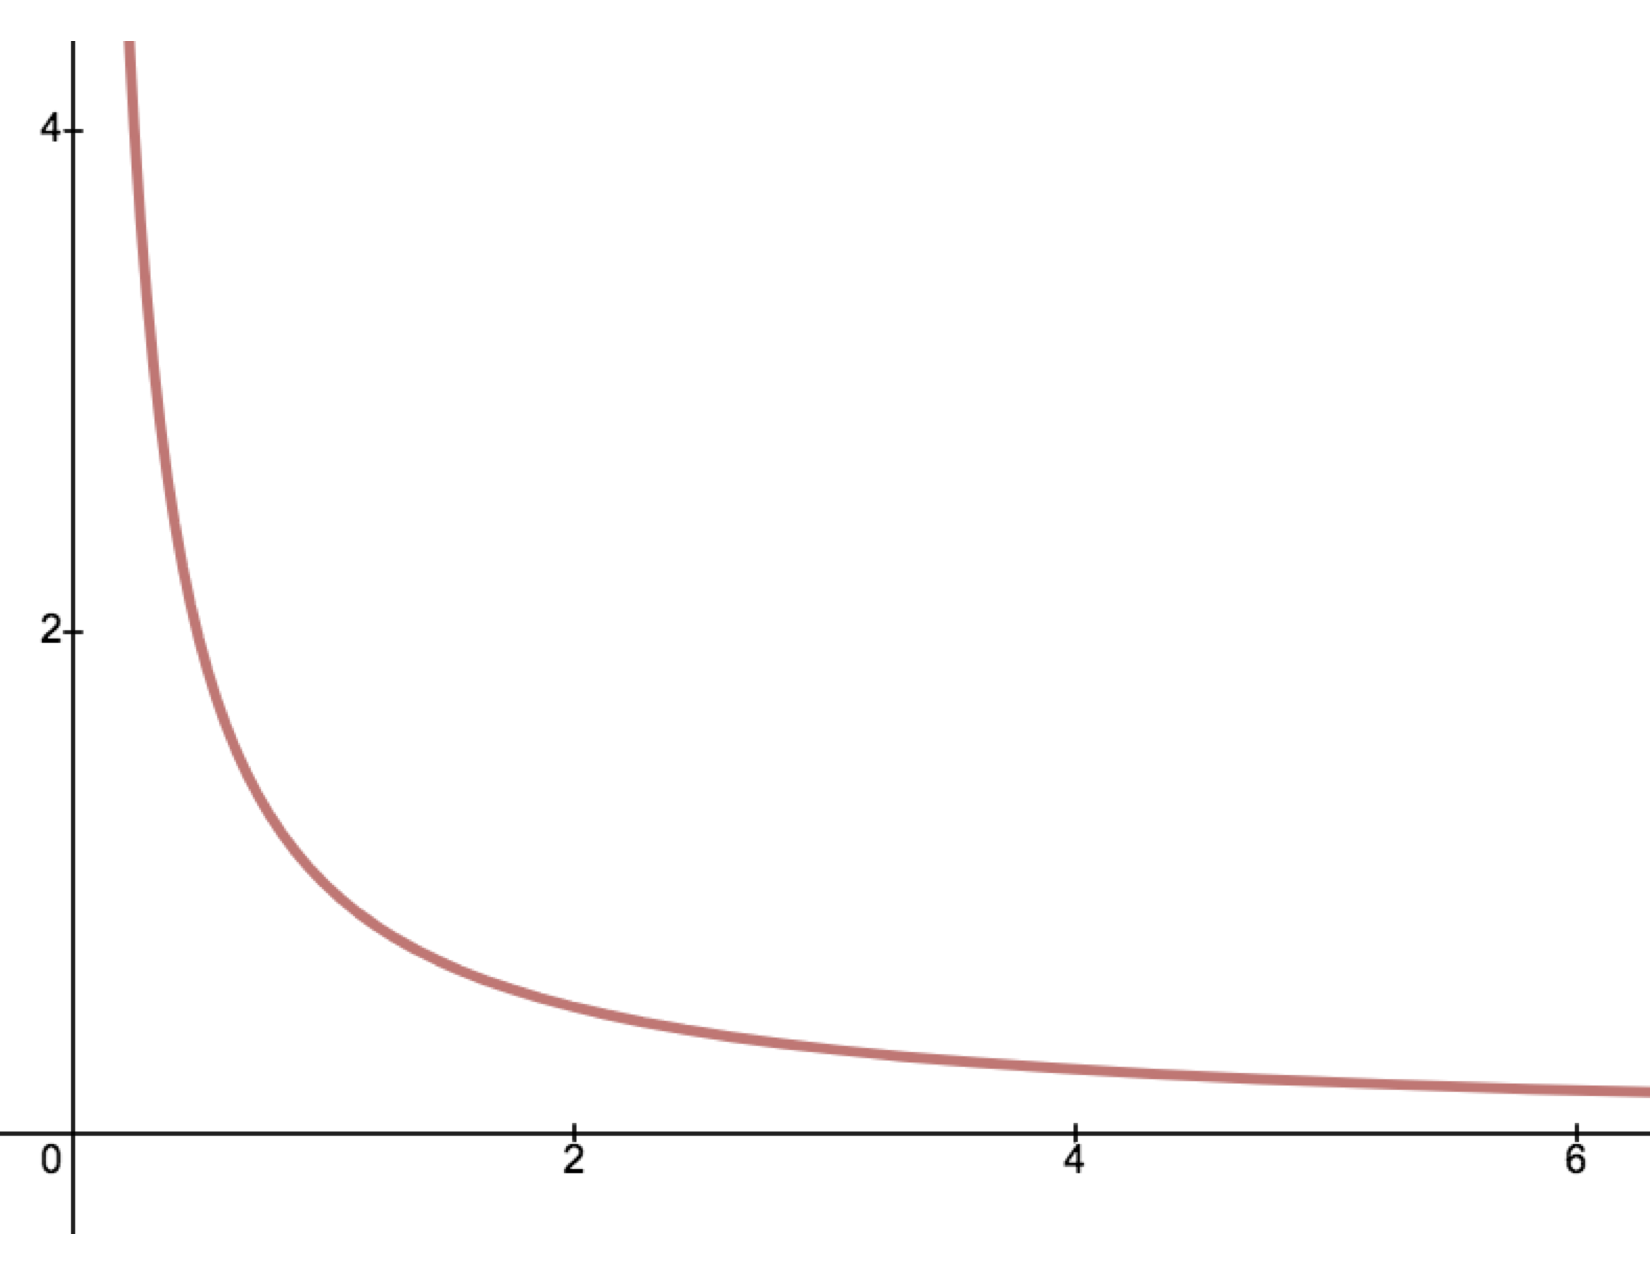
\includegraphics[scale=.3]{nayak_graph_1}
  \end{center}
  \caption{Graph of $f(x)=\frac{1}{x}$}
  \label{fig:2}
\end{figure}

\renewcommand{\thefigure}{3}
\begin{figure}[h]
  \begin{center}
    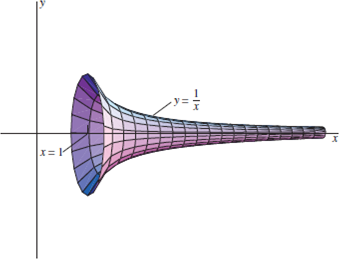
\includegraphics[scale=1]{nayak_graph_2}
  \end{center}
  \caption{Graph of $f(x)=\frac{1}{x}$ on the interval $[1,\infty)$ rotated about the x-axis}
  \label{fig:2}
\end{figure}

\noindent
\textbf{Part I: Solving for Volume}

The standard equation used in calculus for the volume of a curve rotated about the x-axis is: 

\begin{center}
$V=\pi\int_a^b((f(x))^2dx$
\end{center}

In this case, $a=1$, $b=\infty$, and $f(x)=\frac{1}{x}$, so the equation will be: 

\begin{center}
$\pi\int_1^\infty(\frac{1}{x})^2dx=\pi\lim_{b \to \infty} f(x)\int_1^b(\frac{1}{x})^2dx$
\end{center}

We can now solve the improper integral:
\[\pi\lim_{b \to \infty}\int_1^b(\frac{1}{x})^2 dx
= \pi\lim_{b \to \infty}[-x^{-1}]\bigg|_1^b
= \pi\lim_{b \to \infty}[(-\frac{1}{b})-(-\frac{1}{1})]
= \pi \cdot 1
= \pi
\]

Therefore, the volume of the figure is equal to $\pi$. Using the painter example, we can see that he must use $\pi$ cubic units of paint to fill the horn.

	\noindent
	\textbf{Part II: Solving for Surface Area}
		
	We can use another standard calculus formula to solve for the surface area of the figure: 

\begin{center}
$2\pi\int_a^bf(x)\sqrt{1+(f'(x))^2}dx$
\end{center}

Plugging in the known values, $a=1$, $b=\infty$, $f(x)=\frac{1}{x}$, and $f'(x)= -x^{-2}$, we get: 

\begin{center}
$2\pi\int_1^\infty\frac{1}{x}\sqrt{1+(\frac{-1}{x^2})^2}dx=2\pi\int_1^\infty\frac{1}{x}\sqrt{1+\frac{1}{x^4}}dx$
\end{center}

We know intuitively that $\sqrt{1+\frac{1}{x^4}}$ is always greater than 1, so we can say:

\begin{center}
$2\pi\int_1^\infty\frac{1}{x}\sqrt{1+\frac{1}{x^4}}dx>2\pi\int_1^\infty\frac{1}{x}\cdot1dx$
\end{center}

We now solve the improper integral of the second equation:
\[
2\pi\int_1^\infty\frac{1}{x} \cdot 1dx
= 2\pi\lim_{b \to \infty}\int_1^b\frac{1}{x}dx
= 2\pi\lim_{b \to \infty}[\ln{|x|}]\bigg|_1^b
= 2\pi\lim_{b \to \infty}[\ln{|b|}-\ln{|1|}]
= 2\pi\lim_{b \to \infty}[\ln{|b|}]
\]

Since this limit approaches infinity, and since the equation for the surface area of the figure is greater than this limit, the figure’s surface area is also infinite. Therefore, a finite amount of paint will always be unable to cover the full surface of the horn.

\noindent
\textbf{Conclusion}
	
	It is clear why Torricelli’s discovery generated debate among the mathematical community. Many brilliant minds of the time – including Italian astronomer Galileo Galilei, English philosopher Thomas Hobbes, English mathematician John Wallis – struggled with the paradox, as they believed it challenged their ideas of the nature of infinity. After all, how could a figure have a finite volume, and yet have an infinite surface area? Torricelli titled his discovery “Torricelli’s Trumpet,” and it later became better known as Gabriel’s Horn — a reference to the archangel Gabriel. In the Hebrew Bible, the archangel blows his horn on Judgement Day and is related to the divine and the infinite.